\documentclass[reprint,amsmath, amsfonts, amssymb, aps, letterpaper]{revtex4-1}

\usepackage{graphicx,float}
%\usepackage[caption=false]{subfig}
\usepackage{dcolumn}
\usepackage{bm}
\usepackage{enumitem}
\usepackage{tabularx}
\setlength{\extrarowheight}{6 pt}
\newcolumntype{Y}{>{\centering\arraybackslash}X}
\setlist[enumerate]{topsep=0pt,itemsep=-1ex,partopsep=1ex,parsep=1ex}
\usepackage{natbib}
\usepackage{physics}
\usepackage{fancyhdr}
\usepackage{amsthm}
\usepackage{amsmath}
\usepackage{graphicx}
\usepackage{amssymb}
\usepackage{esint}
\usepackage{subfigure}
\usepackage{color}
\usepackage{moreverb}
\usepackage{wrapfig}
\usepackage{physics}
\usepackage{tikz}
\usepackage{siunitx}
%\usepackage{wrapfig}


\begin{document}

\preprint{PHYS CS 15C}
\title{Remotely Operated Vehicle (ROV) with Touch Sensing Control}
\author{Menghang (David) Wang, Weiheng (Frank) Fu, Yiluo Li}
\affiliation{University of California, Santa Barbara, California 93107}

\date{\today}

% Intrigue your audience, connect your project with something people feel more interested in general

% to measure the systematic error, you can try best to maximize the potential one and see if it will genuinely have much effect

\begin{abstract}

\end{abstract}

\maketitle

\section{Introduction}

\section{Touching Pad}
\begin{figure}[h]
\centering
    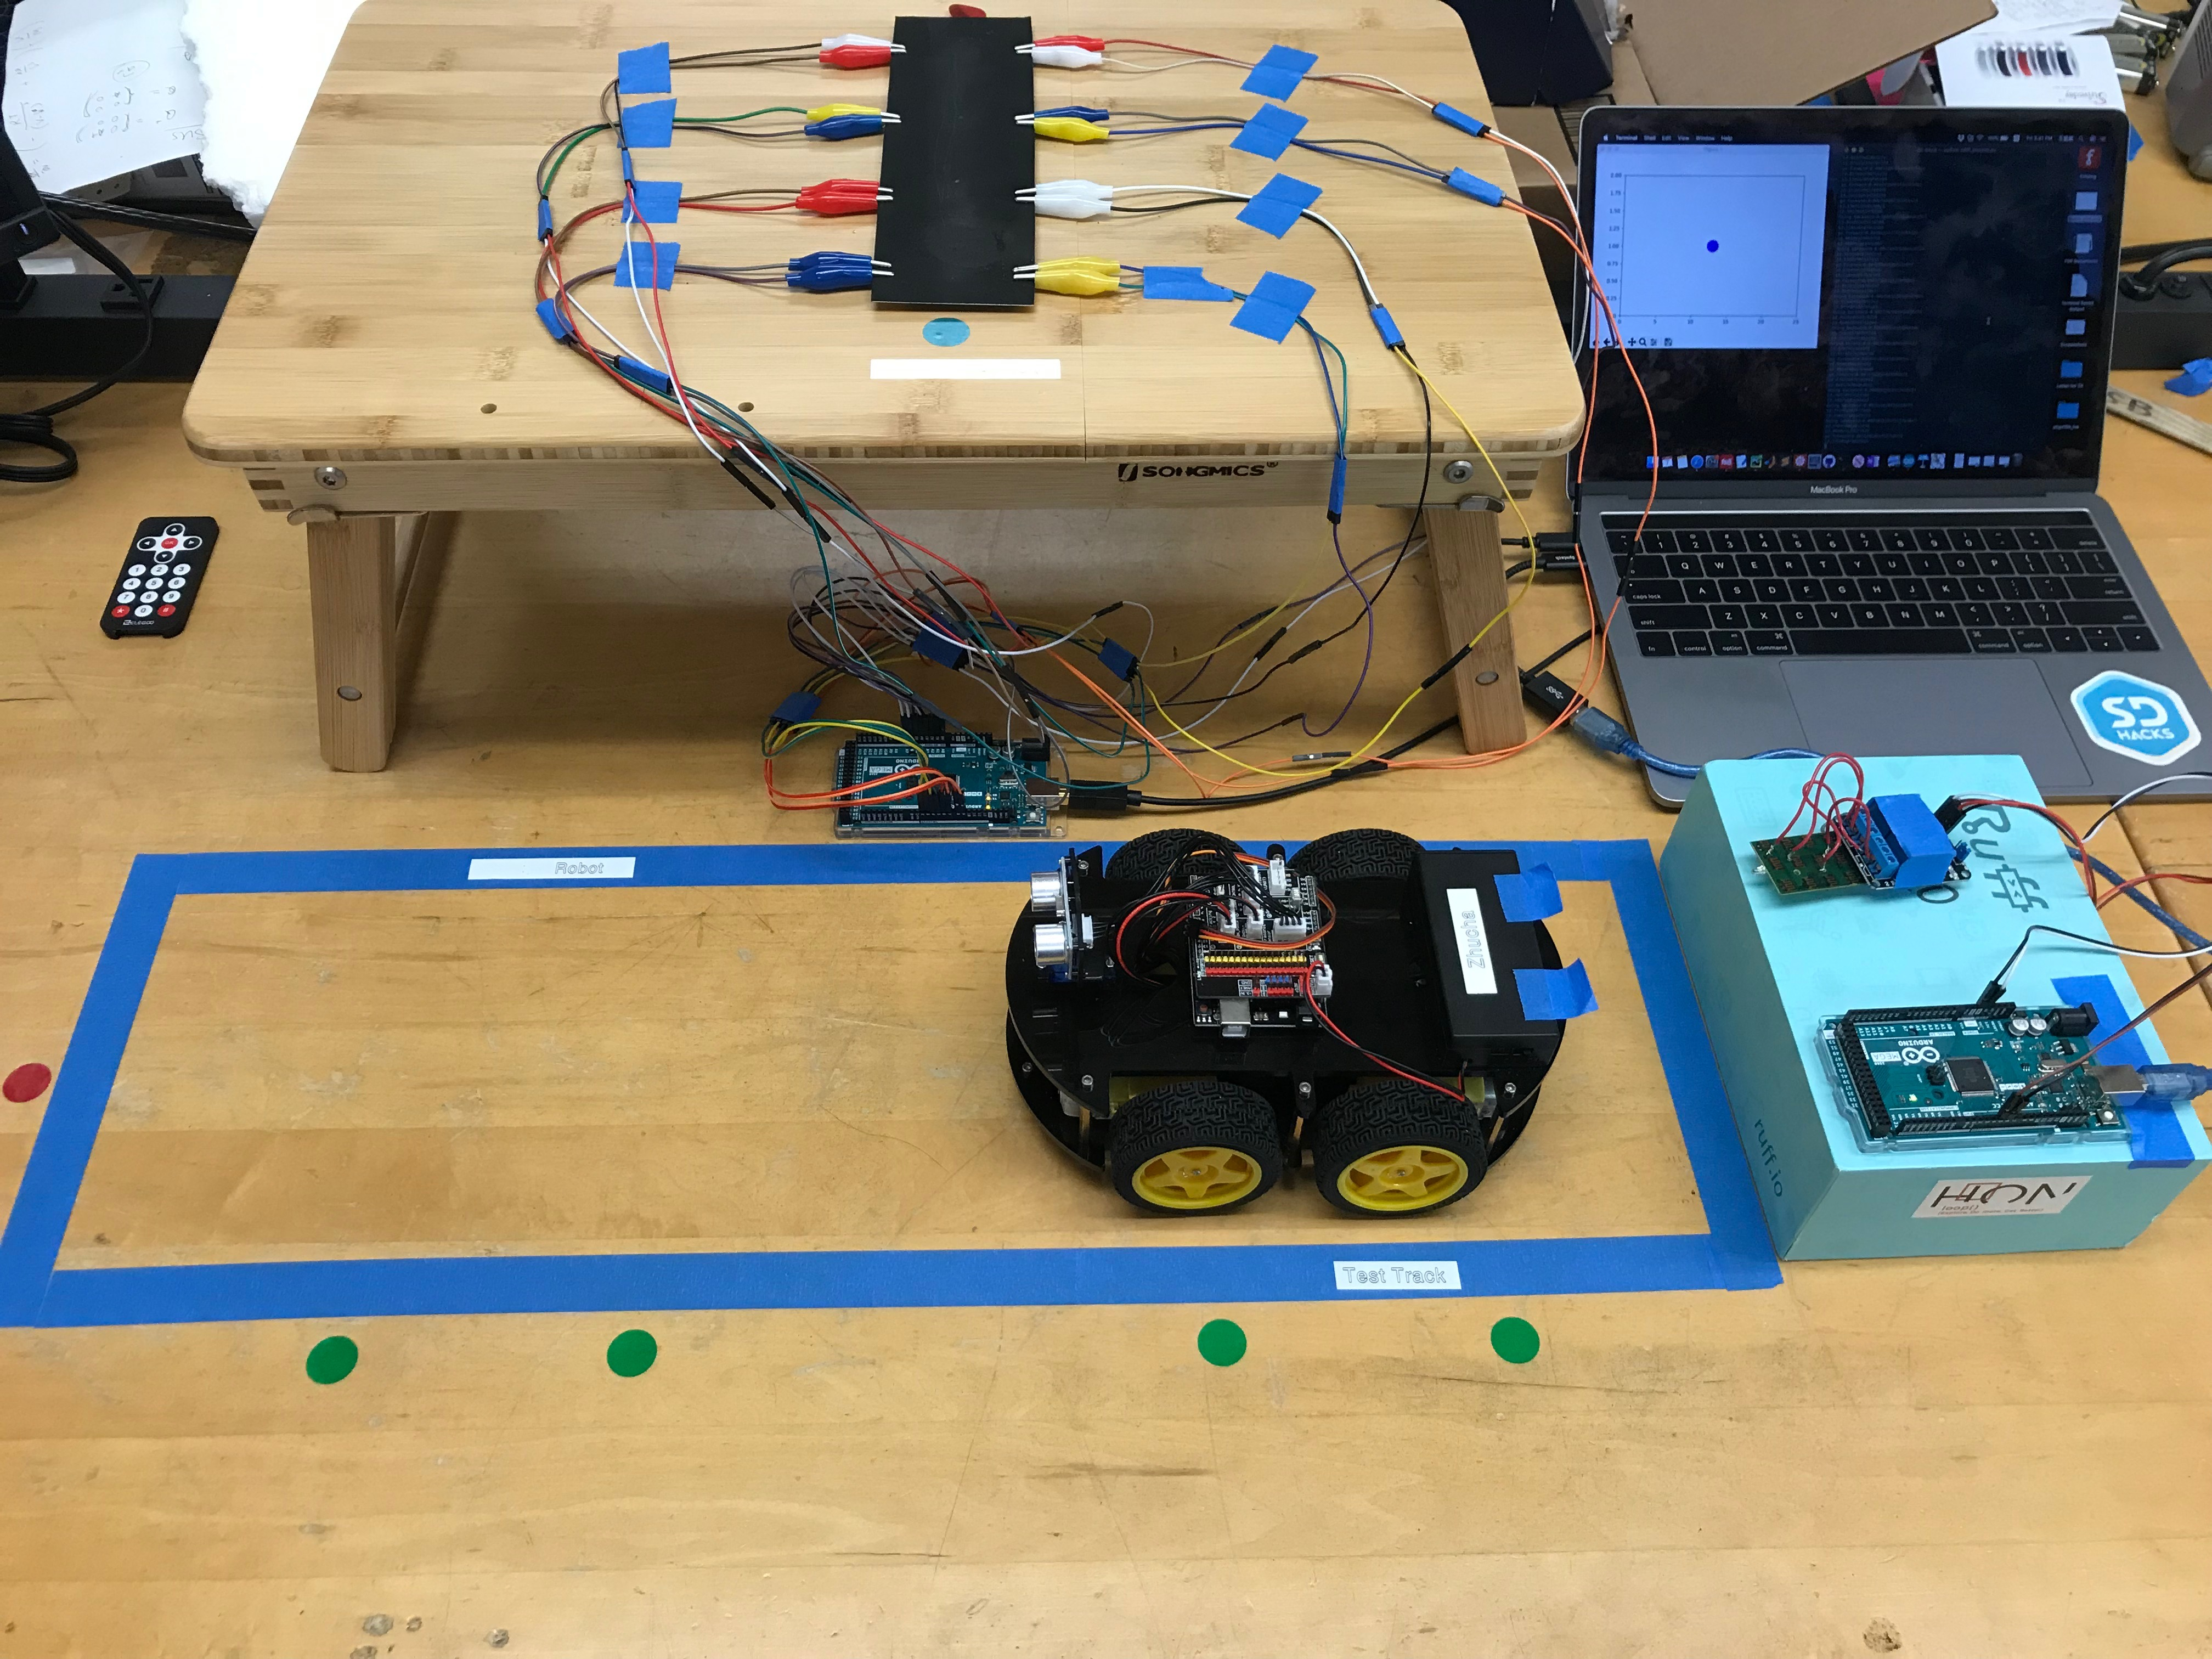
\includegraphics[width=0.5\textwidth]{./figure/setup}     
       \caption{Setup of ROV and touching pad }
    \label{fig::reflect}
\end{figure}
\subsection{Electric sensing principle}
\subsection{Touching pad setup}
\subsection{Measuring procedures}
\subsection{Implementation}

\section{Visualization and Finger Localization}
\subsection{Voltage color-map}
\subsection{Machine learning for finger localization}

\section{Remotely Operated Robot (ROV)}
\subsection{Modules}
\subsection{Control method}
\subsection{Communication with the touching pad}

\nocite{*}
\bibliography{rov}% Produces the bibliography via BibTeX.

\end{document}



